\documentclass[11pt, a4paper]{article}

\usepackage [spanish]{babel}
\usepackage [utf8]{inputenc}
%\usepackage[latin1]{inputenc}para utilizar acentos pero aqui no funciona (en otros si)
\usepackage [T1]{fontenc}
\usepackage{graphicx}
\usepackage{graphics}
\graphicspath{ {images/} } %Para buscar las imágenes en otra carpeta
\usepackage{amsfonts} %Para poder escribir letras como la matriz identidad
\usepackage{mathrsfs} %Para poder escribir letras como la H del el espacio de Hilbert
\usepackage{slashed} % para la d barra cruzada
\usepackage{amsmath}
\usepackage{amssymb}
\usepackage{makeidx}
\usepackage[version=3]{mhchem} %para poder escribir los simpolos atómicos y químicos
%\usepackage{hep}
\usepackage[left=2.5cm,right=2.5cm,top=2.5cm,bottom=2.5cm]{geometry}
\usepackage [labelformat=empty]{caption}
%\usepackage{wrapfig} %for I can use wrapfigure
\usepackage[font={small, up}]{caption}
\usepackage[caption = false]{subfig}
 \usepackage{hyperref} %hipervinculos del índice

\renewcommand{\baselinestretch}{1.15}
\renewcommand{\thefigure}{}

%para aumentar el espacio entre elementos del índice
\usepackage{setspace}

\bibliographystyle{unsrthep}

\begin {document}

\begin{titlepage}

\begin{center}
\vspace*{-1in}
\vspace*{1 cm}
\begin{figure}[htb]
\begin{center}

\includegraphics[scale=1]{Logo1.png}
\end{center}
\end{figure}
\vspace*{2 cm}


{\large MÁSTER EN FÍSICA AVANZADA}\\
\vspace*{0.2in}
{\huge Especialidad en física nuclear y de partículas}\\
\vspace*{0.2in}
\vspace*{0.6in}
\end{center}
\vspace*{-1in}
\begin{center}

\begin{figure}[htb]
\begin{center}

\includegraphics[scale=0.1]{Logo2.jpg} 
\end{center}
\end{figure}
\vspace*{1 cm}

\begin{large}
\textbf{{\large Trabajo final de máster}}\\
\rule{80mm}{0.1mm}\\
%\vspace*{2 cm}

\end{large}
\vspace*{0.2in}
\begin{Large}
\textbf{Diseño de un detector de aguas tritiadas basado en fibras centelleadoras leidas por fotomultiplicadores de silicio} \\
\end{Large}
%\vspace*{0.3in}
\vspace*{2 cm}

\begin{large}
Marcos Martínez Roig\\
\end{large}
\end{center}

\vspace*{0.3in}
%\rule{80mm}{0.1mm}\\
\vspace*{0.1in}
\begin{large}
\begin{flushright}
\item[\bf Tutores:\hspace{4cm} ]\quad  \\ José Díaz Medina\\
Nadia Yahlali Haddou\\
\end{flushright}
\end{large}

\end{titlepage}



\tableofcontents 
\newpage


\section {Introducción}
\paragraph {}
Hoy en día existe un problema que concierne  las  centrales nucleares de fisión, central termoeléctrica,  experimento de física de partículas, etc., e, incluso, en futuras centrales de fusión nuclear y es la creación de altos niveles de radiactividad en estos sitios. Por ejemplo, una central nuclear operando en modo normal puede llegar a emitir alrededor de 300 Tbq/GWy.  Debido a la peligrosidad que ello implica estos deben ser controlados y disminuidos en la medida de lo posible.

\paragraph {}
En concreto, uno de los elementos radiactivos más abundantes generados en estos lugares es el tritio. Debido a las elevadas tasas de radiactividad anteriormente mencionada,es fundamental controlarlo en estas zonas de trabajo para evitar que contribuya a esta cifra ya que un mayor número de emisiónes radiactivas se traduce en una mayor posibilidad de que ello afecte a diversos elementos, entre ellos la salud de las personas.

\paragraph {}
Para que podamos entender la facilidad con la que este se produce el tritio hay que tener en cuenta que este es el tercer isótopo de hidrógeno formado por un protón y dos neutrones. Por un lado, el hidrógeno es uno de los elementos más abundantes de la tierra y, por otro lado, en cualquier lugar de los anteriormente mencionados, se necesita elevar la temperatura para conseguir que, las reacciones en las que se basa su funcionamiento, puedan ocurrir (para abrir el canal de dicha reacción o aumentar la probabilidad de producirse). Como resultado de ello se producen con bastante asiduidad neutrones con energía suficiente para considerase cuasilibres. 

\paragraph {}
Podemos entender entonces que. en estos lugares y en estas condiciones, dada la alta tasa de hidrógeno y neutrones, existe una posibilidad relativamente alta de que aparezca tritio o de que existan diversos elementos que puedan dar lugar a la creación de tritio. Algunos de los principales canales de creación de tritio son la captura neutronica del $^6Li$, $^7Li$, $H$, etc. las cuales se muestran a continuación:

$$\ce{^{6}{Li}} + n \rightarrow T + \ce{^{4}{He}}$$
$$\ce{^{7}{Li}} + n \rightarrow T + \ce{^{4}{He}} + n$$
$$\ce{^{1}{H}} + 2n \rightarrow T $$

Según nuestro planteamiento también será más facil todavía que se produzca deuterio, segundo isótopo del hidrógeno (compuesto por un protón y un neutrón). Esto es verdad pero ello no nos importa para nuestro objetivo debido a que el deuterio no es un isótopo radiactivo.

\paragraph {}
Como hemos dicho, el tritio es el tercer isótopo del hidrógeno compuesto por un proton y dos neutrones. Se trata de un elemento radiactivo con un periodo de semidesintegración de 12.32 años, en concreto, un emisor $\beta^-$ de baja energía que emite electrones según la siguiente reacción:

$$T \rightarrow \ce{^{3}{He}} + e^- + \overline{\nu}_e$$

Donde lo que ha ocurrido es que uno de los neutrones que conforman el tritio se ha desintegrado (a partir de una interacción débil) de acuerdo a una desintegración $\beta^-$ en un protón, un electrón y un antineutrino electrónico:

$$n \rightarrow p + e^- + \overline{\nu}_e \qquad \rightarrow \qquad (pnn)_T\rightarrow (ppn)_{^3He} + e^- + \overline{\nu}_e $$

La existencia de este antineutrino electrónico es impuesta por la conservación del numero leptónico, en concreto el número leptónico de la familia del electrón ($L_e$). En la práctica no tenemos la posibilidad de detectar esta partícula ya que interacciona muy debilmente con la materia ($\sigma \propto 10^{-42} \quad cm^2$) y por tanto con el material que conforma nuestro detector (en concreto fibras centelleadores BCF-12). Es decir, esta partícula escapa sin interaccionar con el detector y en su lugar solo detectamos su ausencia, es decir, la no conservación de ciertas cantidades físicas como energía, momento, número leptónicos, etc. en la totalidad de las partículas detectadas.

\paragraph {}
Por tanto solo tenemos la posibilidad de detectar el isotopo $^3He$, isótopo estable, y el electrón. Hay que tener en cuenta que, aunque el isótopo hijo de la reacción de desintegración del tritio, $^3He$, sea estable (presenta una vida media infinita, es decir, no se desintegra) realmente este se encontrará en un estado no estacionario, es decir, no se encuentra en un autoestado de su hammiltoniano, sino en un estado que puede expresarse como una la suma de autoestados del hamiltoniano. Como consecuencia, tras la desintegración $\beta^-$ del tritio tendremos una posterior desexcitación del $^3He$ que producirá fotones con varias energías bien definidas, fotones que podremos observar en nuestro detector. En resumen obtendremos un espectro de desintegración del tritio junto a un espectro típico de rayos X, espectro idealmente discreto pero experimentalmente gaussiano debido a incertidumbre de los aparatos de medida.

\paragraph {}
Dado que el $^3He$ presenta una masa muy superior a la de los electrones, por conservación de energía y momento podemos observar que el $^3He$ apenas se movera del sitio donde ha ocurrido la reacción. Por tanto nos centraremos en la detección del electrón. En la imagen 1 podemos apreciar el espectro energético de los electrones emitidos en la desintegración del trito.

\begin{figure}[hbtp]
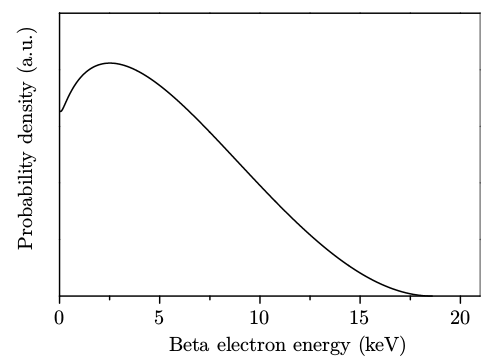
\includegraphics[scale=0.4]{Espectro.png}
\centering
\caption{\textbf{Imagen 1}.-Espectro energético}
\end{figure}

Como era de esparar este presenta la forma típica de un espectro energético de una desintegración $\beta$. Podemos observar que estos poseen una energía máxima de 18,6 keV, una energía promedio de 5,7 keV y una moda (valor más probable) lígeramente inferior a la energía promedio, entorno a 4,5. Con estos valores de energía podemos apreciar que la energía de radiación del tritio es la más pequeña observada hasta el momento en los isótopos. Como consecuencia el electrón presentará un recorrido libre medio muy corto, del orden de 3-5 mm en el aire y de 5-6 $\mu m$ en la fibra centelleadora.

\paragraph {}
El problema actual reside en que los mecanismos de detección y monitorización de tritio utilizados en la actualidad, en concreto en centrales nucleares, que será el objetivo final del detector que pretendemos desarrollar en el grupo experimental internacional denominado \textit{Tritium}, son métodos lentos o con un alto umbral de detección. 

\paragraph {}
Por ejemplo, entre los métodos más empleado actualmente en centrales nucleares, esta el método de detección de aguas tritiadas por medio de centelleo líquido. Este es el metodo más indicado para la detección de partículas beta de energía muy pequeña porque, como ya se ha visto al analizar el espectro energético de los electrones que conforman la radiación $\beta$ del tritio estos presentan un recorrido libre medio muy pequeño (del orden del mm o $\mu m$, dependiendo del medio). Dado que solo contribuye a la medida (con una probabilidad aceptable) las emisiones que han tenido lugar a una distancia del detector inferior al recorrido libre medio la forma más efectiva de conseguir que un mayor volumen de la fuente radiactiva contribuya a la señal y que un mayor volumen del detector se encuentre a una distancia adecuada de la fuente radiactiva es disolviendo este detector con el líquido radiactivo (en nuestro caso agua tritiada), y esto solo se puede conseguir utilizando detectores líquidos de partículas beta, como liquido centelleador. 

\paragraph {}
El método de centelleo líquido consiste en tomar una muestra del líquido radiactivo, agua tritiada en nuestro caso, diluirla (habitualmente al 50\%) con el líquido centelleador y medir los fotones emitidos por este líquido centelleador, a partir de los cuales podremos determinar los electrones emitidos por la muestra de agua tritiada y detectados por el líquido centelleador siempre y cuando este líquido centelleador este previamente calibrado. Sin embargo para ello se necesita tomar una muestra y llevarla al laboratorio para el correspondiente estudio. En resumen se trata de un proceso de detección de agua tritiada basado en metodos offline que ralentizan la monitorización dilatando el resultado hasta varios dias desde la toma de la muestra. 

\paragraph {}
Tras cada análisis, la muestra de agua tritiada y líquido centelleador son inseparable y por tanto no reutilizable.  Este debe de ser tratado como residuo peligroso ya que, aunque el análisis desvele que el agua tritiada esta libre de tritio (presente una actividad suficientemente baja para ser tratada como material no radiactivo), esta contiene tolueno, presente en el líquido centelleador y, por tanto, debe de ser procesada de manera segura. También necesita operarios especializados manipulen estas muestras, poniendo en peligro su salud (referencia del artículo "sampling tritiated water vapor from the atmosphere by an active system using silica gel").

\paragraph {}
El objetivo final de \textit{Tritium}, sobre el cual tratará mi futura tésis, es desarrollar un detector de aguas tritiadas que permita realizar la monitorización del tritio \textit{in situ} a tiempo real. Por tiempo real entendemos una dilatación temporal máxima de 10 minutos desde la toma de la muestra (ya que se necesita un tiempo mínimo para poder discernir la señal del background, el cual dependera, entre otras cosas, de la configuración del sistema de detección). Además el prototipo desarrollado no necesitará de la presencia de personal especializado que intervenga en el proceso de monitorización de aguas tritiadas, agilizando y abaratando el método de monitorización, además de excluir posibles errores humanos. El método simplemente requerirá continuas calibraciones al cabo de un tiempo determinado para asegurar el correcto funcionamiento del dispositivo. 

\paragraph {}
La dificultad aquí residirá en conseguir extraer esta señal tan pequeña ($keV$) y tener estadística suficiente para poder discernirla del fondo radiactivo en un tiempo tan pequeño. Los trabajos \textit{in situ} con configuraciones del detector similares (centelleador + contador de fotones) realizados hasta la fecha que utilizan el concepto de tiempo real solo han conseguido obtener una señal en el límite del MeV ("citar referencía a la tesis"). Estos estan basados principalmente en solidos centelleadores y tubos fotomultiplicadores (PMT) a diferencia de nuestro experimento que consta de fibras centelleadoras (que detectan la radiación beta del tritio y la convierten en fotones) y tubos fotomultiplicadores o fotomultiplicadores de silicio (que detectan estos fotones y los convierten en electrones que conformarán la señal del sistema). 

\paragraph {}
En mi opinion el uso de fibras centelleadores es una mejor elección ya que presentan un mayor volumen activo con el que detectar el la radiación del tritio  sin necesidad de utilizar líquido centelleador el cual, como he mencionado anteriormente, produce residuos peligrosos además del coste del líquido centelleador no reutilizable. Además las fibras centelleadoras presentan un mayor abanico de posibilidades en cuanto a la elección de las distintas estructuras de las mismas. Nuestro experimento se centrará en la utilización de SiPM aunque también contemplará el uso de PMT. 

\paragraph {}
Hay que tener en cuenta que si existen diseños que logran llegar a límites del orden del Bequerelio en un tiempo de 3 minutos, aunque estos estan basados en configuraciones totalmente distintas, como por ejemplo un sistema, conformado por un láser y cavidades espectroscópicas en forma de anillo, en el cual se pretende buscar la existencia de resonacias y relacionar las frecuencias a las que estas ocurren con la concentración de tritio presente en la muestra. ("citar referencia Tritiated water detection in the 2,17 micrometros spectral region by cavity ring down spectrsocpy"). Sin embargo este es un estudio totalmente diferente ya que necesita de un acondicionamiento y control exhaustivo de las condiciones del sistema para el correcto funcionamiento del láser, encareciendo la construcción y mantenimiento del mismo y dificultando la existencia de este en sitios como centrales nucleares, es decir, es una aplicación que no persigue un mismo fín.

\paragraph {}
Para conseguir extraer una señal tan pequeña con la mayor eficiencia posible estudiaremos diversas configuraciones experimentales para conseguir obtener la mas adecuada de acuerdo a nuestro objetivo experimental. Además realizaremos en todo momento detecciones en coincidencia, lo cual nos permitira eliminar en gran medida el fondo radiactivo del experimento. Las configuraciónes que pretendemos abarcar en el experimento son: 
\begin{itemize}
\item {}
Por un lado estudiaremos cual es la mejor elección para las estructuras de fibras centelleadores. Estudiaremos las ventajas y desventajas que presenta la utilización clads en las fibras (recubrimiento de la fibra centelleadora para evitar la fuga de fotones de centelleo y poder dirigir estos de manera opticamente aceptable hasta el contador de fotones). Las fibras que utilizaremos, BCF-12, consiguen esto con una eficiencia del... (((((((incluir porcentaje)))))))))  ) 
\item {}
Por otro lado estudiaremos cual es la mejor elección para un contador de fotones. Las posibilidades contempladas en el experimento serán SiPM o PMT. Veremos cual es más adecuado ya que cada una presenta una serie de características mejores como la eficiencia de fotodetección (PDE) de los SiPM sobre la de los PMT pero otras tantas peores como la dependencia con la temperatura más acusada en los SiPM que en los PMT.
\end{itemize}

\paragraph {}
También se realizarán una serie de simulaciones del experimento previas al desarrollo del mismo utilizando el programa "Geant 4", desarrollado por el cern, con el objetivo de ver que es el que deberíamos esperar teóricamente de nuestros resultados. Estas simulaciones nos permitiran comparar nuestros resultados experimentales con los datos simulados para ver hasta que punto nuestro experimento dista del modelo teórico seguido, lo cual nos permitira a su vez comprobar la fiabilidad de este modelo teórico y corregir posibles erratas del mismo. También nos permitirá ver que posibles modificaciones podemos realizar en el experimento para obtener un mejor resultado.

\paragraph {}
El grupo experimental \textit{Tritium} es un grupo internacional compuesto por tres paises: Portugal, Francia y España; En concreto intervienen las universidades de...  El proyecto que planteamos en este grupo es demasiado extenso para una trabajo de fín de master ya que se necesitan años para conseguir resultados concluyentes y, como ya se ha mencionado anteriormente, será la base de mi futura tésis. En este trabajo de fin de máser únicamente nos centraremos en los primeros pasos de este gran proyecto, el cual ha empezado recientemente y, afortunadamente, me ha permitido estar en este desde el inicio.

\paragraph {}
Dividiremos este trabajo en cinco partes:
\begin{itemize}
\item{} En primer lugar realizaremos una calibración de los SiPM, paso fundamental antes de poder obtener cualquier medida del experimento. La finalidad de este paso es poder catalogar la magnitud de la medida del sistema que estamos obteniendo con este instrumento, algo fundamental en física. No se necesita realizar una calibración de los PMT, paso igualmente importante al anterior, ya que esta fue realizada recientemente. 
\newline
En último lugar se realizara una comparación de estas dos posibles configuraciónes para ver cual es la más adecuada y que, por tanto, presentará el diseño final del detector.

\item{} En segundo lugar se realizará un pequeño estudio sobre las fibras centelleadoras. En primer lugar se determinará cual es la forma adecuada de actuar a la hora de manipular fibras centelleadoras, elemento más sensible de los utilizados en el experimento, presentando el procedimiento final de como preparar un bunch de fibras centelleadoras con resultado opticamente aceptable. Finalmente se utilizarán distintas estructuras de las mismas para ver cual nos permite obtener la señal del agua tritiada  más óptima. 

\item{} En tercer lugar se describirán cada una de las configuraciones que conforman los distintos prototipos y se presentaran las medidas realizadas sobre los mismos de forma que, aun sin ser el diseño final, nos ayudarán para orientarnos experimentalmente, a determinar posibles fallos y mejoras del diseño. Estos serán mas fáciles de determinar a pequeña escala, actuando de manera constructiva, y nos permitirá discernir que mejoras presenta un prototipo sobre otro. 

\item{} En cuarto lugar se presentarán las simulaciones realizadas con el programa de Geant4, programa desarrollado por el cern capaz de realizar simulaciones muy detalladas de experimentos, principalmente de física de partículas. En este punto se presentaran las simulaciones realizadas tanto para los prototipos como para posibles diseños finales. Esto nos permitirá ver que posibles mejoras podemos incluir a nuestro experimento y en que puntos difieren los resultados obtenidos con las simulaciones con los resultados obtenidos en los distintos experimentos de los prototipo.

\item{} Se presentará un último punto donde se expondrán las conclusiones alcanzadas durante la completitud del trabajo y se comentaran posibles partes del experimento que queden inconclusas o inacabadas o puntos interesantes y que serán propuestos a futuros estudios que habrá que realizar durante la tésis.
\end{itemize}

\newpage

\section {Calibración de los fotomultiplicadores de silicio (SiPM)}
\paragraph {}
El fotomultiplicador de Silicio es un dispositivo de detección de radiación relativamente nuevo en el mercado que surge como alternativa al tubo fotomultiplicador. Este consiste en un array bidimensional formado por multiples pixels independientes y alimentados en paralelo (mismo voltaje operacional para cada uno) a un voltaje tal que les permita estar en modo Geiger. Cada uno de los pixels actua como un APD (fotodiodos de avalancha).

\paragraph {}
Cuando detectan un foton estos pixels producen una cascada de pares electrón hueco que pasará a formar parte de la señal del sistema de detección, la cual estará formada por la suma de las señales de cada pixel que han detectado un fotón para cada instante de tiempo. Idealmente cada pixel únicamente puede detectar un fotón. Dado que poseen una alta eficiencia de fotodetección los SiPM son utilizados como contadores de fotones, especialmente para señales débiles.

\paragraph {}
Debido a ello presenta una serie de propiedades distintas a los convencionales tubos fotomultiplicadores que lo hacen ideal para unas situaciones y no tanto para otras, como por ejemplo su tamaño compacto, inmunidad a campos magnéticos, electrónica sencilla, alta eficiencia de detección de fotones (especialmente adecuado para nuestro experimento), buena linealidad, dependencia con la temperatura, alta ganancia a menor voltaje de alimentación y, por extensión, menor consumo, tiempo de respuesta corto y, por extensión, buena resolución temporal.

\paragraph {}
Hay que tener en cuenta que los SiPM son detectores de estado sólido y, por extensión, presentan ruido térmico, ruido que se verá amplificado por el hecho de estar operando en modo Geiger. Este ruido es denominado corriente oscura (Dark counts) y su forma se ve reflejada en la siguiente imagen:

\begin{figure}[hbtp]
\centering
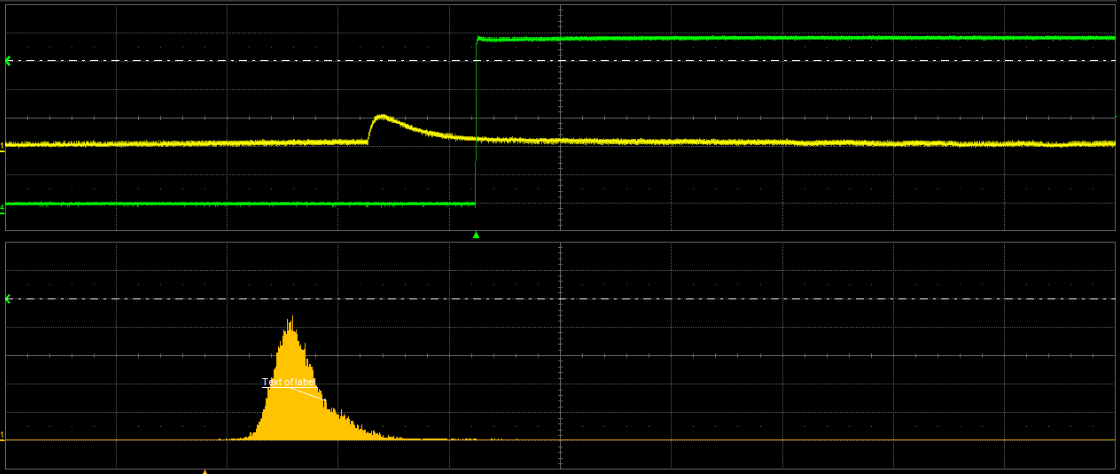
\includegraphics[scale=0.2]{pedestal.png}
\caption{\textbf{Imagen 2}.- Dark counts}
\end{figure}


%\paragraph {}
Cuando trabajemos con detectores de estado sólido debemos trabajar en condiciones de voltaje operacional y temperatura óptimas para poder medir con el detector ya  que, estas cuentas oscuras dependen de estas magnitudes y pueden llegar a ser tan numerosas que absorban por completo la señal del sistema. También podemos reducir su importancia sobre la medida con ayuda de triggers, por ejemplo, medir únicamente cuando la señal de entrada del sistema este activa (si se conoce este intervalo de tiempo). En cualquier caso siempre se deberá realizar una medida del pedestal (sin señal de entrada) para tener en cuenta el número y características de los eventos que van a contribuir a la señal sin proceder de la misma y utilizar esta información para el posterior análisis. 

\paragraph {}
En esta sección nos proponemos desarrollar un método de compensación para las variaciones de la ganancia de un fotomultiplicador de silicio derivadas de la temperatura a partir de variaciones derivadas del voltaje de alimentación del SiPM (voltaje de desertización), de ahora en adelante llamado voltaje operacional. 

\paragraph {} 
En concreto utilizaremos el modelo S13360-1375CS de hamamatsu, ya que será el modelo que utilizaremos en el prototipo del experimento. Se ha elegido este modelo ya que presenta una eficiencia de fotodetección máxima entorno a los 450 nm, que corresponde aproximadamente a la longitud de onda del azul, 435 nm y, en concreto, se asemeja bastante con el máximo de la energía reemitida por las fibras centelleadoras BCF-12, 435 nm, encargadas de detectar la radiación $\beta$ del agua tritiada en nuestro experimento como puede apreciarse en la siguiente imagen. Con esto conseguiremos que la señal sea tan grande como sea posible, algo fundamental ya que, como ya se ha mencionado, una de las principales dificultados del experimento es que estamos intentando extraer una señal muy pequeña.

\begin{figure}[htb]
\centering
{
%\subfloat[PDE]
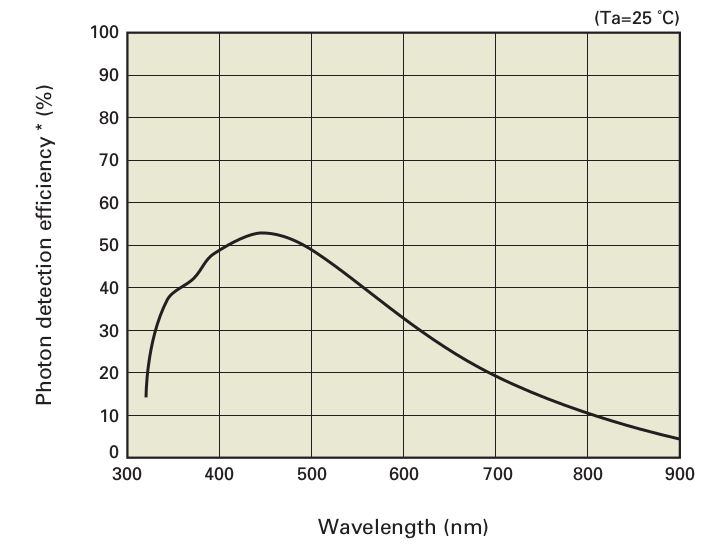
\includegraphics[scale=0.2]{PED.png} 
}
{
%\subfloat[Espectro de emisión]
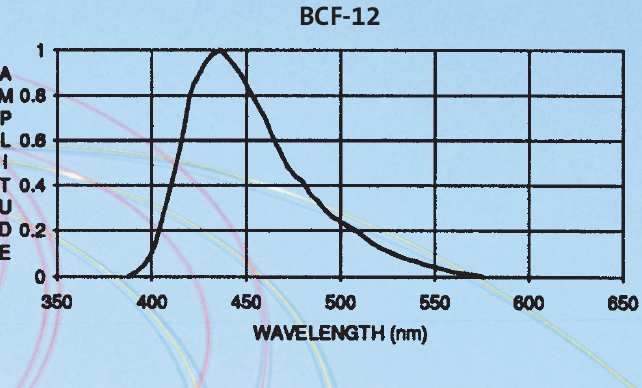
\includegraphics[scale=0.25]{EmisionBCF12.png} 
}
\caption{\textbf{Imagen 3}.-PDE y espectro de emisión respectivamente}
\end{figure}

%\paragraph {}
%IMAGEEEN JUNTA

La forma de abordar este método de compensación de la ganancia ha sido el siguiente:
\begin{itemize}
\item {} 
Por un lado se ha realizado una calibración de la ganancia frente a la temperatura obteniendo su relación de dependencia. Para ello se ha necesitado la utilización de un sistema de control de temperatura. En concreto se ha utilizado un sistema de la marca DYCOMETAL, (modelo CCM 81) que permite controlar temperatura y humedad relativa con una precisión de 0.1 grados y  0.5\% respectivamente.

\item {} Por otro lado se ha realizado una calibración de la ganancia frente al voltaje operacional obteniendo su relación de dependencia. Para obtener este voltaje operacional se ha utilizado un electrómetro de la marca KEITHLEY, en concreto el modelo 6517B, el cual presenta una resolución inferior al mV, más que suficiente para considerar este totalmente constante ya que se necesitan mayores modificaciones para que estas sean apreciables en la ganancia.

\item {} Finalmente, a partir de estas dos dependencias determiandas, se ha obtenido la ecuación de dependencia entre voltaje operacional y temperatura que nos determine una ganancia constante  y se ha realizado un test de comprobación para esta relación.
\end{itemize}

\paragraph {}
El objetivo final de este estudio será mantener la ganancia del fotomultiplicador de silicio constante ante variaciones involuntarias de la temperatura a partir de variaciones voluntarias con el voltaje operacional. Esta es una correción fundamental para el objetivo final del detector ya que de lo contrario (no) obtendríamos alertas de fugas de tritio cuando estas no (si) han ocurrido, cuando, en realidad, lo único que ha ocurrido ha sido una modificación de temperatura.

\newpage

\subsection {Equipo y montaje experimental} 
\paragraph {} 
Para llevar a cabo esta caracterización de los SiPM se ha necesitado de cierta instrumentación la cual se especifica a continuación:

\begin{itemize}
\item {} En primer lugar se necesitaba una \textbf{cámara de control de temperatura}. 
\newline
Dado que la cámara existente en el laboratorio del IFIC no estaba configurada tuvo que utilizarse la camara que se encontraba en el IFIMED. Esta cámara (marca DYCOMETAL, modelo CCM 81) se ve reflejada en la imagen cuatro.

\begin{figure}[htb]
\centering
{
%\subfloat[PDE]
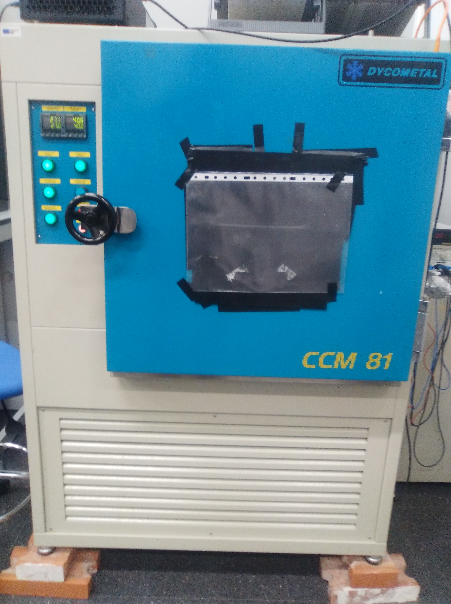
\includegraphics[scale=0.15]{SistemaTemperatura.png} 
}
{
%\subfloat[Espectro de emisión]
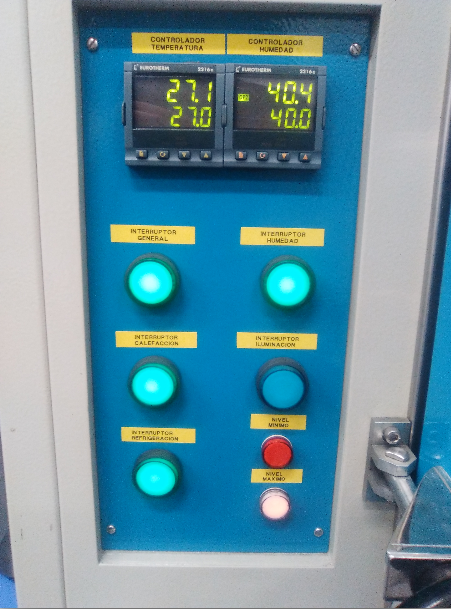
\includegraphics[scale=0.15]{PanelTemperatura.png} 
}
\caption{\textbf{Imagen 4}.-Sistema de control de temperatura}
\end{figure}

Este sistema dispone de un panel de control con el que poder especificar la temperatura y humedad a la que queremos trabajar en el interior de la cámara. Sin embargo, para asegurar el correcto funcionamiento de la cámara debiamos trabajar siempre en la zona 1 de acuerdo al diagrama de fases existente en la ficha técnica de la cámara, mostrado en la imagen cinco. Posee un interior metálico que nos permite una rápida estabilidad ante posibles cambios de las condiciones en su interior y, además, actua a modo de jaula de Faraday. 

\begin{figure}[htb]
\centering
{
%\subfloat[Espectro de emisión]
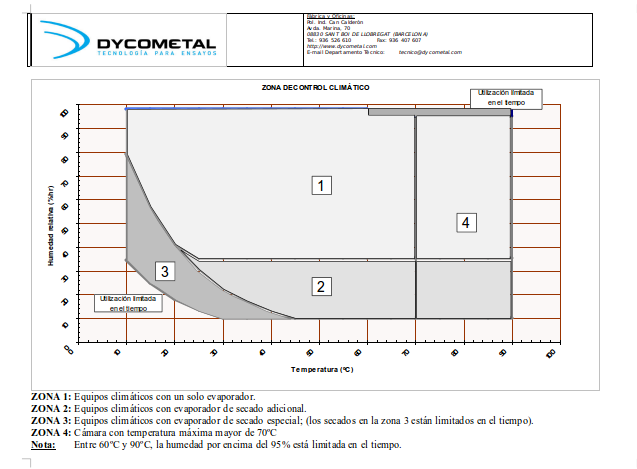
\includegraphics[scale=0.15]{FichaTecnica.png} 
}
{
%\subfloat[Espectro de emisión]
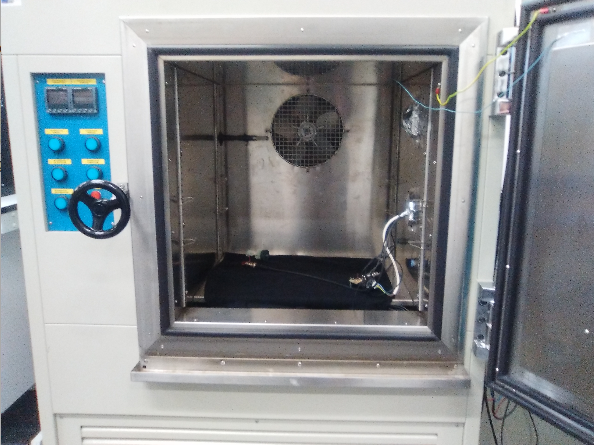
\includegraphics[scale=0.15]{InteriorTemperatura.png} 
}
\caption{\textbf{Imagen 5}.-Interior del sistema y diagrama de fases}
\end{figure}

Su incertidumbre se encontraba en 0.1 grados para la temperatura y 0.5\% para la humedad relativa. Estas incertidumbres se determinaron observando la oscilación  máxima en la pantalla del panel de ambos parámetros tras llegar a la estabilidad en el interior de la cámara.

\paragraph {}
En el interior de esta cámara se encontraba nuestra fuente que proporcionaba la señal de entrada del sistema que pretendíamos medir con el SiPM, el propio SiPM, la tarjeta de conversión intensidad-voltaje y cableado que hacía posible la interacción con estos dispositivos. Además hay que tener en cuenta que esta cámara no actuaba como caja negra, por lo que para conseguir reducir la posible entrada de luz del exterior se taparon todas las posibles fisuras del sistema con cinta metálica, se apagó la luz del laboratorio, se cerraron ventanas y, ademas, se cubrió el experimento con una tela negra especial. Con todo esto conseguiamos reducir el background del sistema hasta un nivel adecuado.

\item {} En segundo lugar se necesitabamos instrumentos nos permitiesen alimentar tanto el SiPM como la tarjeta de conversión intensidad-voltaje. Se utilizo  un \textbf{electrometro} (marca KEITHLEY, modelo 6517B) para alimentar el SiPM y un \textbf{generador de tensión} (marca ISO-TECH, modelo...) para alimental la tarjeta de conversión, ambos reflejados respectivamente en la imágen seis.

\begin{figure}[htb]
\centering
{
%\subfloat[Espectro de emisión]
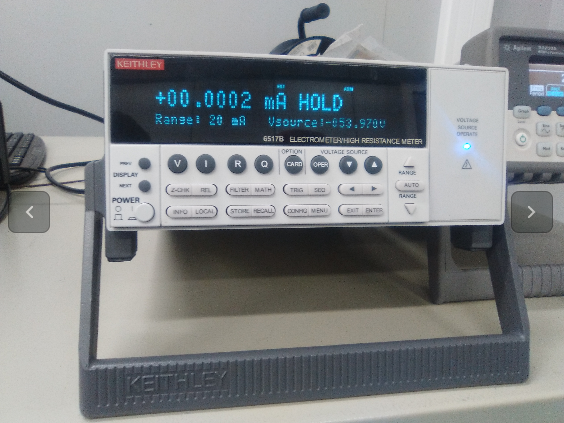
\includegraphics[scale=0.2]{KEITHLEY.png} 
}
{
%\subfloat[Espectro de emisión]
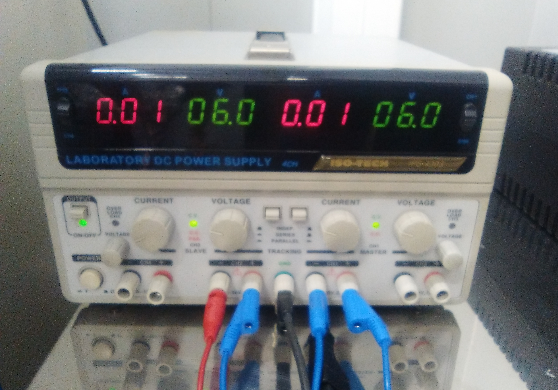
\includegraphics[scale=0.2]{ISO-TECH.png} 
}
\caption{\textbf{Imagen 6}.-Electrómetro y Generador de tensión}
\end{figure} 

Se utilizo el electrómetro para el SiPM ya que este dispone de rango de voltajes mayor, necesario para alimentar al SiPM. Por el contrario, el ISO-TECH solo dispone de una tensión máxima de ((((())))))) insuficiente para alimentar al SiPM pero suficiente para alimentar la tarjeta. Poseen una resolución inferior inferior al milivoltio e inferior a 0.1 voltios respectivamente, suficiente para considerarlos constantes ya que las ganancias que dependen de estos (ganancia del SiPM y de la tarjeta respectivamente) necesita variaciones superiores para modificarse de forma apreciable.

\item {} En tercer lugar se necesitaba una \textbf{fuente} que simulase los fotones de la fibra centelleadora. 
\newline
Se utilizo un \textbf{diodo LED} que emitía fotones con una longitud de onda de 435 nm, correspondiente al azul. Este es la longitud de onda que necesitabamos en nuestro experimento para calibrar el SiPM ya que corresponde a la longitud de onda a la cual el espectro de emisión de las fibras centelleadoras BCF-12 tiene su máximo. Este diodo LED puede verse reflejado en la imagen siete.

\begin{figure}[hbtp]
\centering
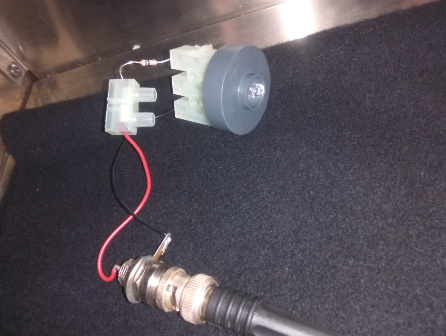
\includegraphics[scale=0.25]{LED.png}
\caption{\textbf{Imagen 7}.- LED}
\end{figure}

%\newpage
\item {} En cuarto lugar, para alimentar este diodo LED se necesito un \textbf{generador de señales} (marca Agilent, modelo 33250A). Este se puede observar en la imagen ocho.

\begin{figure}[hbtp]
\centering
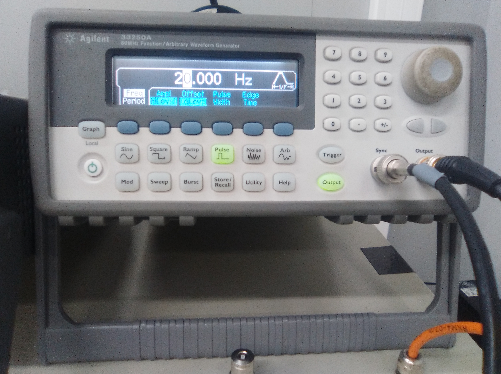
\includegraphics[scale=0.2]{GeneradorOnda.png}
\caption{\textbf{Imagen 8}.- Generador de señales}
\end{figure}

\newpage
Este generador de señales nos permite especificar la forma del pulso que pretendemos proporcionar y sus características. En concreto alimentaremos el diodo LED con un pulso cuadrado. Los parámetros que nos permite especificar el generador de señales para un pulso de esta forma son frecuencia (o periodo), high level (o amplitud), low level, offset, anchura del pulso y tiempo de decaimiento. Para nuestro estudio los valores de estos parámetros que nos daban un mejor resultado desde el punto de vista experimental fueron una frecuencia de 20 Hz, high level de 2.275 V, low level de 1 V, offset de 1.638 $V_{dc}$, anchura del pulso de 12 ns y tiempo de decaimiento de 5 ns.

\paragraph {}
Este generador de señal nos proporciona una segunda señal denominada señal de sincronización la cual podemos utilizar como trigger para determinar el instante de tiempo en el que se activa la señal.

\item {} En quinto lugar utilizamos un \textbf{SiPM} para detectar los fotones emitidos por el LED 
\newline
En concreto se utilizo el modelo S13360-1375CS de hamamatsu, que es un fotomultiplicador cerámico de silicio  que presenta una ganancia teórica de $G=4 \cdotp 10^6$ y una eficiencia de fotodetección teórica del 50\% a 25 grados y $V_{ov}=V_{op}-V_{bd}=3V$.  

\paragraph {}
Esta compuesto por un total de 285 pixels de 75 $\mu m$ cada uno dando lugar a una superficie total activa de 1.3 $mm^2$ frente a su superficie total que es de 6 $mm^2$. Este puede verse reflejado en la imagen nueve.

\begin{figure}[hbtp]
\centering
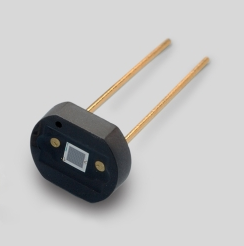
\includegraphics[scale=0.25]{SiPM.png}
\caption{\textbf{Imagen 9}.- SiPM}
\end{figure}

\item {} Hay que tener en cuenta que el SiPM nos proporciona un pulso de intensidad a la salida y  necesitamos convertir este en un pulso de voltaje para, de esta forma, poder introducirla al osciloscopio para realizar el posterior análisis. Para ello emplearemos en sexto lugar una \textbf{tarjeta conversora} de intensidad en voltaje que puede verse reflejada en la imagen diez. 

\begin{figure}[hbtp]
\centering
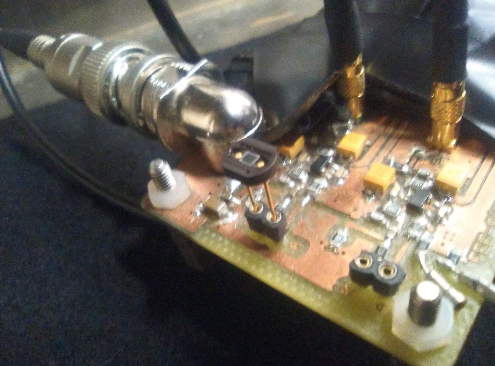
\includegraphics[scale=0.2]{tarjeta.png}
\caption{\textbf{Imagen 10}.- Tarjeta}
\end{figure}

\newpage
\item {} Finalmente vimos que, únicamente alimentando la tarjeta, antes de alimentar el SiPM y la led, obteníamos una perturbación externa a nuestro experimento. Esta se presenta en la imagen once. 

\begin{figure}[hbtp]
\centering
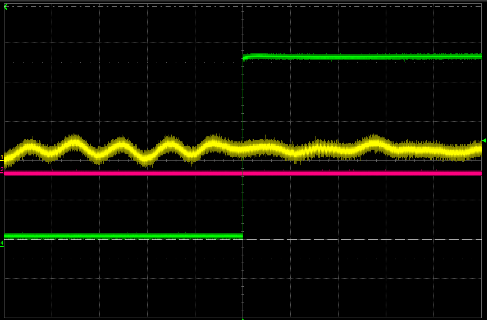
\includegraphics[scale=0.2]{ruido.png}
\caption{\textbf{Imagen 11}.- Perturbación}
\end{figure}

Se intento caracterizar esta señal de perturbación ajena a nuestro experimento y, a priori, de origen desconocido. Tenía una amplitud máxima de 4 mV y una frecuencia demasiado irregular para ser determinada. 

\paragraph {}
Con la presencia de este ruido no podíamos realizar medidas ya que introducía una componente de ruido tal que estropeaba por completo el resultado de la medida. Se suposo que procedía de las conexiones de los distintos intrumentos a la red eléctrica, ya que el IFIC posee una toma de tierra bastante irregular. Se dispuso de un \textbf{filtro pasa banda} con el fin de eliminar este ruido. Este puede verse reflejado en la imagen doce

\begin{figure}[htb]
\centering
{
%\subfloat[Espectro de emisión]
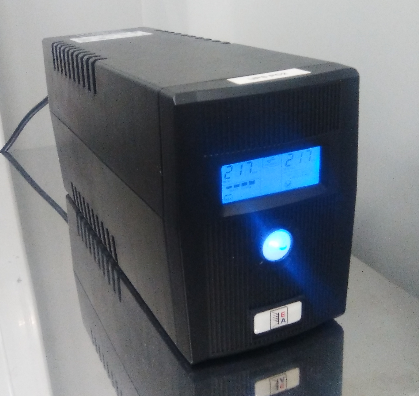
\includegraphics[scale=0.2]{Filtro1.png} 
}
{
%\subfloat[Espectro de emisión]
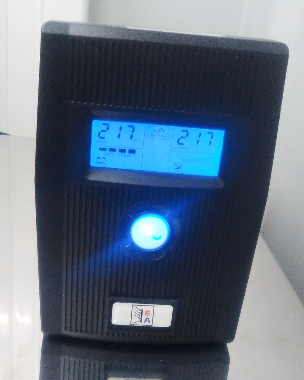
\includegraphics[scale=0.2]{Filtro2.png} 
}
\caption{\textbf{Imagen 12}.-Filtro pasa banda}
\end{figure} 

\item {} Como se ha mencionado anteriormente, necesitamos, entre otras cosas, uso de una \textbf{manta negra} especial que apantallase la entrada de fotones del exterior, ya que el sistema de control de temperatura no actuaba  como caja negra. Esta manta negra puede verse en la imagen trece.

\begin{figure}[hbtp]
\centering
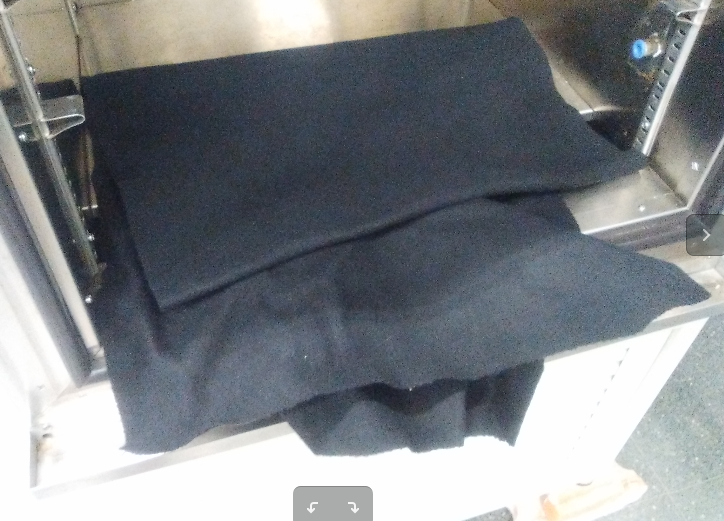
\includegraphics[scale=0.2]{MantaNegra.png}
\caption{\textbf{Imagen 13}.- Manta negra especial}
\end{figure}


Una alternativa podría haber sido introducir una caja negra en el interior del sistema de control de temperatura y introducir el diodo Led, el SiPM y la tarjeta en su interior. Sin embargo de esta forma no conseguimos un control de la temperatura y humedad en su interior.

\end{itemize}



\newpage

\subsection {Calibración tarjeta}
\paragraph {}
La tarjeta empleada en el sistema, que puede verse en la imagen 10, es una tarjeta reciclada un un proyecto anterior. Esta consiste de dos entradas distintas donde podemos conectar dos SiPM distintos. Hay que tener en cuenta que esta tarjeta únicamente nos servirá para el prototipo ya que este solo contendrá un bunch de fibras centelleadoras y nos bastará con un único SiPM. Sin embargo el detector final contendrá un mayor número de fíbras centelleadoras y, por extensión, para funcionar de la forma más optimizada posible, necesitará disponer de un mayor número de SiPM.

\paragraph {}
Esta tarjeta esta formada por...%TFM bueno. Página 33

\paragraph {}
Presenta una ganancia teórica de 1500 pero, para mayor seguridad, se realizao una calibración de la misma. Para ello se introdujo una señal de....	

\subsection {Análisis de datos}
\paragraph {}
En resumen, en nuestra prueba de calibración de los SiPM tenemos una caja que actuará como jaula de faraday, con temperatura y humedad controlada y apantallada en lo posible de la luz del exterior. 

\paragraph {}
En su interior tendremos un diodo LED que emite fotones a $\lambda=435$, un SiPM, el cual emitirá un pulso de intensidad cada vez que detecte uno o más de estos fotones con cada uno de sus pixels y una tarjeta que convertirá este pulso de intensidad en un pulso de voltaje. Finalmente llevamos este pulso de voltaje a un osciloscopio (marca TELEDYNE LECROY, modelo WwaveRunner 625Zi) para poder ser analizado. 

\paragraph {}
Una vez en el osciloscopio, la señal que recibíamos cuando se encendía el diodo led era similar a la de la imagen catorce.

\begin{figure}[hbtp]
\centering
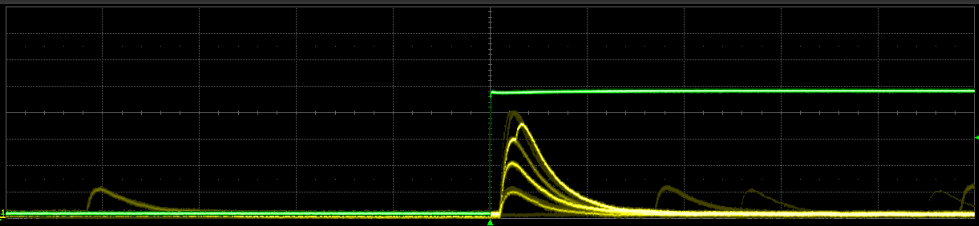
\includegraphics[scale=0.2]{PulsoSalida.png}
\caption{\textbf{Imagen 14}.- Pulso de salida}
\end{figure}

Donde se a activado el modo persistencia del osciloscopio con el objetivo de comparar señales de distintas alturas. Estas señales corresponden a distinto número de pixels activados en cada instante de tiempo ya que, como hemos dicho anteriormente, la señal de salida del sistema es la suma de las señales de cada pixel que se ha activado. La señal de color verde corresponde a la señal de sincronización que actua como trigger.

\paragraph {}
El objetivo ahora es calcular la ganancia del sistema. Dado que únicamente existen dos ganancias en el sistema (SiPM y tarjeta) y hemos medido la ganancia de la tarjeta en la sección anterior, determinando la ganancia total podremos determinar la ganancia del SiPM. 

$$G_{tot}=G_{SiPM} \cdotp G_{card} \longrightarrow G_{SiPM} = \frac{G_{tot}}{G_{card}}$$

Para medir la ganancia total simplemente realizamos una integral del area de cada uno de los pulsos de salida del sistema y conservamos el resultado en un histograma. De esta forma lo que estamos consiguiendo es un histograma de las cargas de los pulsos. La ventana temporal sobre la que se integra es aproximadamente una división, que equivale a 500 ns. Esta se ajusta con bastante precisión al pulso, algo muy importante para evitar la introducción de background.

\paragraph {}
Dado que idealmente el pulso de cada pixel es igual, el histograma que estamos obteniendo deberían ser deltas de dirac equiespaciadas. Sin embargo hay que tener en cuenta que la cascada que produce cada uno de estos fotones detectados en cada pixel esta sometido a fluctuaciones estadísticas. Además los propios instrumentos de medidas empleados tienen una incertidumbre inherente. Hay que tener en cuenta que tambień tenemos distintas fuentes de background, como dark counts (ruido térmico), fotones de luz del exterior, etc. 

\paragraph {}
Como resultado de todo esto, lo que obtendremos seran un conjunto de gaussianas equiespaciadas. En la imagen quince puede verse el resultado de una toma de datos de 25000 eventos a 25 grados, 60\% de humedad y $V_{ov}=3V$

\begin{figure}[hbtp]
 \centering
 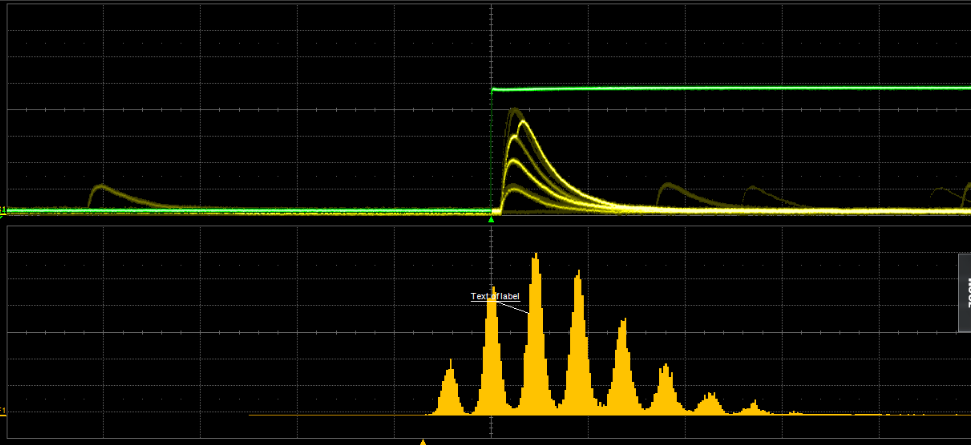
\includegraphics[scale=0.2]{Analisis.png}
 \caption{\textbf{Imagen 15}.- Análisis}
 \end{figure}

Donde cada uno de estos picos corresponde a la carga de sucesivos número de pixels activados (uno, dos, etc.). El primer pico no debe tenerse en cuenta en el análisis ya que este corresponde al pedestal (cero pixels activados). Su origen es debido a la existencia de las cuentas ocuras.
 
\paragraph {}  
Ahora únicamente desarrollamos una macro en ROOT (programa de análisis de datos desarrollado por el CERN) que, utilizando la librería TSpectrum (librería especialmente diseñada para el análisis de histograma) nos permita obtener la ganancia del sistema. Su forma de proceder es la siguiente:
\begin{itemize}
\item {} Primero la macro lee el fichero de datos y lo guarda en una variable de tipo histograma. La macro se detiene cuando no encuentra más valores para leer.

\item {} A continuación, a partir de una función de la librería TSpectrum, busca en este histograma y devuelve el número de gaussianas que ha encontrado y su posición.

\item {} Ahora ajusta todos los datos del histograma a una recta y solo se queda con las gaussianas, cuya norma sobrepasa en altura a esta recta. El objetivo de este paso es que, en casos muy concretos (temperatura alta o luz del laboratorio encendida) tenemos mucho ruido y, aparece un fondo el cual, el programa ajusta a una gaussiana y, por extensión, calcula la ganancia de manera incorrecta. Un ejemplo de esto se muestra en la imagen dieciseis.

\begin{figure}[hbtp]
\centering
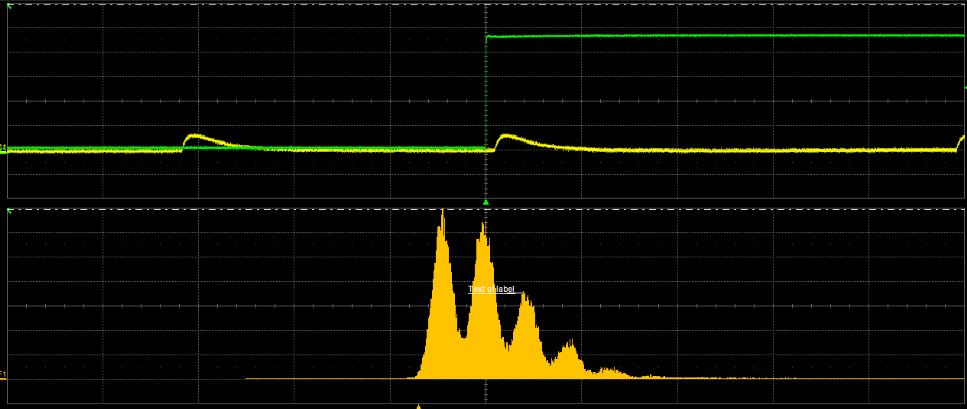
\includegraphics[scale=0.2]{fondogaussiano.png}
\caption{\textbf{Imagen 16}.- Espectro con mucho fondo}
\end{figure}

\newpage
\item {} Seguidamente, ajustamos el espectro a una recta mas una suma de n gaussianas, donde n es el número de gaussianas que superan la recta (calculado en el paso anterior). La necesidad de utilizar una recta es debido a que siempre vamos a tener dark counts y otro tipo de bakcground que se verán reflejados en una linea base en el histograma como puede verse en la imagen quince. Podemos apreciar en la imagen diecisiete que el ajuste es relativamente bueno.

\begin{figure}[htb]
\centering
{
%\subfloat[Espectro de emisión]
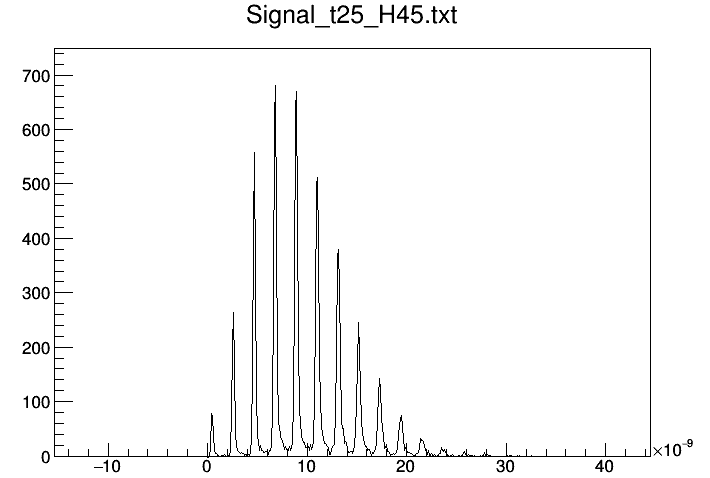
\includegraphics[scale=0.2]{Espectroo.png} 
}
{
%\subfloat[Espectro de emisión]
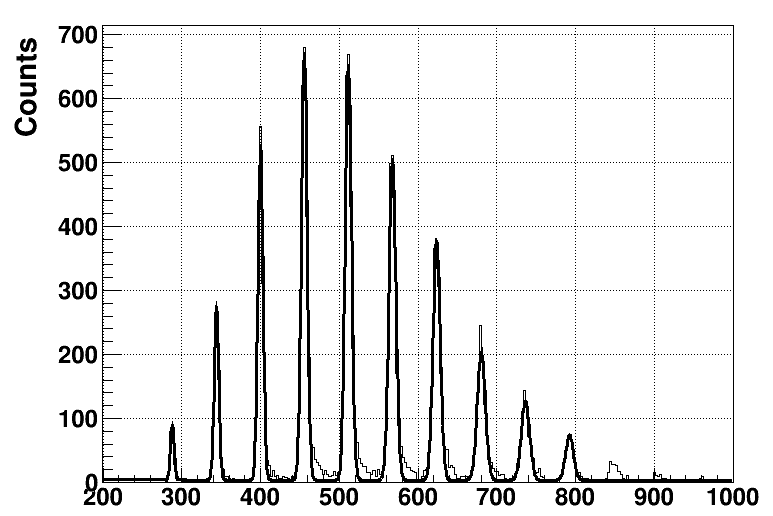
\includegraphics[scale=0.2]{AjusteEspectro.png} 
}
\caption{\textbf{Imagen 17}.-Espectro y ajuste}
\end{figure} 

\item {} Dado que se ha observado que, aun con el tercer paso, existen situaciones límites en que el background sigue superando esta recta, se ha incluido un paso en la macro en la cual se acepta por teclado uno a uno los picos que serán utilizados en el análisis. Además la macro calcula la resolución de cada gaussiana y la resolución total, obtenida a partir de la suma cuadrática de la resolución de cada gaussiana. Los valores habitualmente encontrados en los análisis se encuentran sobre 1.5\% y 5\% respectivamente, valores más que aceptables.

\item {} Finalmente la macro los ordena según su posición en el espectro y calcula la ganancia por dos caminos:
	\begin{itemize}

	\item {} Por un lado se ha calculado la distancia promedio entre sucesivas gaussianas del espectro. 
	$$Q = G N_\gamma + Q_0 \longrightarrow \Delta Q= Q_{N_\gamma} - Q_{N_\gamma -1}=G N_\gamma+ Q_0 - G(N_		\gamma -1) - Q_0 = G$$
	Podemos observar que este cálculo corresponde a la ganancia. Hay que tener en cuenta que se han 			empleados factores de conversión para convertir la posición del pico (inicialmente en unidades de			tensión, V) en unidades de carga (coulomb). En concreto se ha utilizado el factor $\frac{1}{eR}$, 			donde R es la resistencia del osciloscopio, 50 $\Omega$ y e es la carga del electrón.
	
	\item {} Por otro lado se ha ajustado a una recta las posiciones horizontales de estas gaussianas en el 	espectro frente a el número de pixels. Esto nos da la siguiente ecuación:
	$$Centro\_pico(V) = GeRN_\gamma + k_0$$	
	Donde R y e significan lo mismo. Vemos por tanto que apartir del valor de la pendiente podemos obtener 		el valor de la ganancia. La imagen dieciocho muestra un ejemplo de ajuste entre posiciones de 				gaussianas y número de pixels para el caso de 25 grados, humedad de 45\% y $V_{ov}=3V$. Podemos 			observar que existe	un acuerdo excelente, algo que ocurria prácticamente en la totalidad de los casos. 		Este gráfico presenta barras de error pero no son apreciables a esta escala.
		
	\begin{figure}[hbtp]
		\centering
		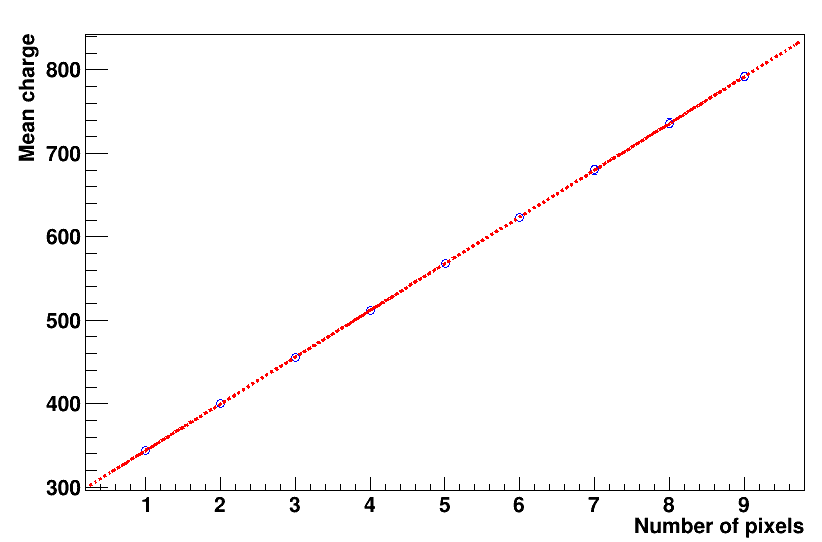
\includegraphics[scale=0.2]{FitPosicionPixels.png}
		\caption{\textbf{Imagen 18}.- Ajuste posicón frente a pixels}
		\end{figure}
			
	
	\end{itemize}
	
Para este caso concreto las ganancias obtenidas por los dos caminos anteriores son respectivamentente:
$$G_1= 6.38938 \cdot 10^8 \pm  6.38938 \cdot 10^8 $$  
$$G_2=7.18235 \cdot 10^8 \pm 6.88392 \cdot 10^6$$
Por extensión, las ganancias del SiPM calculadas por cada camino son (aproximadamente) 
$$G_1= 4.25958 \cdot 10^5 \pm 4.259 \cdot 10^4$$  
$$G_2= 4.78823 \cdot 10^5 \pm 4.5893 \cdot 10^4$$
donde los errores se han obtenido por propagación. Hay que tener en cuenta que el primer método siempre posee errores mayores. Estas se encuentran un orden de magnitud por debajo de la ganancia teórica, con un error relativo de... Esto es debido a...

\paragraph {}
Dado que, en la practica, las gaussianas no estan perfectamente equiespaciadas debido a errores e incertidumbres consideraremos como más fiable el segundo método ya que se trata de un método más formal. 


\end{itemize}

\subsection {Calibración en temperatura}
\paragraph {}
Ahora que ya sabemos calcular la ganancia del SiPM a partir de una toma de datos procedemos a determinar la dependencia que presenta el SiPM con la temperatura. En concreto nos interesa determinar el comportamiento de su ganancia cuando varía la temperatura. Para ello realizaremos una serie de medidas a distintas temperaturas y, para cada una de ellas, calcularemos la ganancia a partir del metodo expuesto en el punto anterior.

\paragraph {}
Nos centraremos en el rango de temperatura entre 15 grados, que es el mínimo que nos permitía llegar el sistema de control de temperatura y 41 grados, que, suponemos, será el límite al que llegará nuestro futuro detector en la práctica. Es decir, este rango de temperaturas será equivalente a las temperaturas a las que estará sometido nuestro detector debido a las condiciones climáticas del lugar. Realizaremos pasos de 2 grados entre cada medida realizando un total de 14 medidas. Únicamente realizaremos medidas de 15000 eventos ya que son más que suficiente para obtener un espectro suficientemente suave. 

\paragraph {}
Para automatizar este proceso procedemos a desarrollar una macro en ROOT que realice este ajuste. Esta macro se divide en dos partes:
\begin{itemize}
\item{} Por un lado posee un bucle en el que, en cada paso, abre el fichero correspondiente a una temperatura, empezando por la mínima (15 grados) realiza todo el estudio anterior y guarda ganancia y temperatura con sus errores en 4 vectores respectivamente. En cada paso aumenta 2 grados la temperatura y pasa a leer el siguiente fichero.

\paragraph {}
Hay que tener en cuenta que, como se dijo anteriormente, el sistema de control de temperatura debe de estar en la zona uno del diagrama de fases existente en la ficha técnica. Esto implico que, para medidas inferiores a 27 grados necesitamos aumentar la humedad en un 5\% a cada medida (humedad del 45\% para 25 grados, 50\% para 23 grados, etc.). Esto no tiene mayor importancia ya que se vio que la ganancia del SiPM no se ve afectada de forma apreciable ante modificaciones de la humedad de este tamaño.

\paragraph {}
La incertidumbre en la temperatura viene dada por la oscilación en el valor de la temperatura observada directamente en el panel de control del sistema. La oscilación observada fue en todo momento de 0.1 grados, una incertidumbre totalmente inapreciable tanto a nivel visual en la gráfica como a nivel de variación de la ganancia.

\item {} Por otro lado, partiendo de estos 4 vectores de dimensión 14 en nuestro caso (igual al número de ficheros que ha leido) que contienen ganancia, temperatura y sus errores de forma ordenada la macro realiza un ajuste lineal. El ajuste obtenido se presenta en la imagen diecinueve.

\begin{figure}[hbtp]
\centering
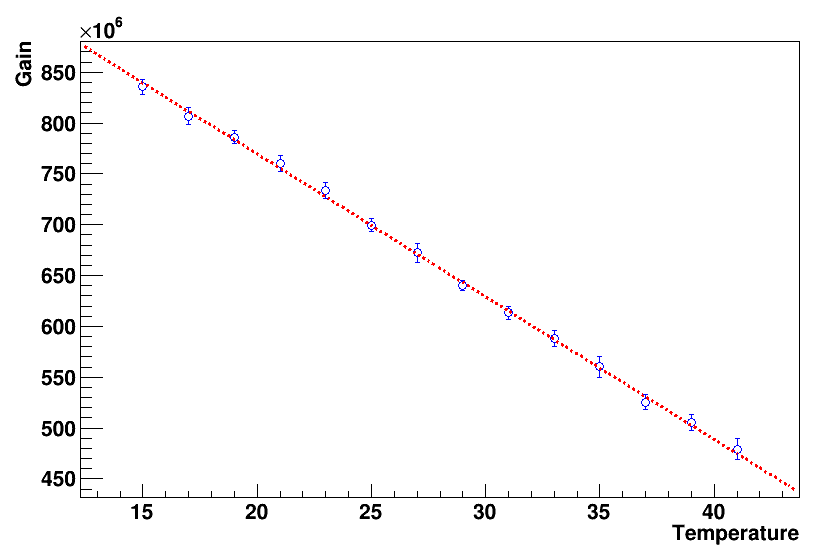
\includegraphics[scale=0.2]{Dependenciatemperatura.png}
\caption{\textbf{Imagen 19}.- Ganancia frente a temperatura}
\end{figure}

Podemos observar la existencia de un comportamiento lineal casi perfecto en un rango de temperatura de 26 grados. Esta es una propiedad que caracteriza al SiPM, una muy buena linealidad en su comportamiento frente a modificaciones en varias magnitudes.

\paragraph {}
Podemos observar que la existencia de un decrecimiento del valor de la ganancia del SiPM a medida que aumenta la temperatura. Esto es debido a que....

\paragraph {}
La ecuación obtenida en este ajuste $G=aT+b$ toma los siguientes valores: 
\begin{itemize}
\item{} $a=-1.40308 \cdot 10^7 \pm 2.71545 \cdot 10^5$ $T^{-1}$
\item{} $b=1.05001 \cdot 10^9 \pm 7.69711 \cdot 10^6$ $T^{-1}$
\end{itemize}

Esta es un resultado importante, no por el valor numérico, sino porque será la base que utilizaremos para conseguir la compensación de la ganancia.
\end{itemize}



\subsection {Calibración en Voltaje de operación}
\paragraph {}
De forma totalmente análoga procedemos a determinar el comportamiento del SiPM, en concreto de su ganancia, frente al voltaje operacional. Para ello realizaremos una serie de medidas a distintos voltajes operacionales y, para cada una de ellos, calcularemos la ganancia a partir del metodo expuesto anteriormente. 

\paragraph {}
Nos centraremos en el rango de voltajes entre el voltaje break down, $V_{BD}= 50.97$ V, que es el mínimo voltaje en valor absoluto a partir del cual nos encontramos en modo Geiger y $V_{BD}+5V$, que, suponemos, será un intervalo suficiente para compensar la ganancia acorde con el intervalo de temperaturas que hemos medido. Realizaremos pasos de 0.2 V entre cada medida realizando un total de 25 medidas. De nuevo unicamente realizaremos medidas de 15000 eventos ya que son más que suficiente para obtener un espectro suficientemente suave.

\paragraph {}
Para automatizar este proceso procedemos a desarrollar una macro en ROOT que realice este ajuste. Análogamente esta macro poseerá dos partes:
\begin{itemize}
\item{} Por un lado posee un bucle en el que, en cada paso, abre el fichero correspondiente a un voltaje operacional, empezando por el mínimo ($V_{op}=V_{BD}$) realiza todo el estudio anterior y guarda ganancia y voltaje operacional con sus errores en 4 vectores respectivamente. En cada paso aumenta 0.2 V el voltaje operacional y pasa a leer el siguiente fichero. 

\paragraph {}
En este estudio, a diferencia del estudio de la temperatura, la incertidumbre en el voltaje viene dada por la precisión del electrómetro (milivoltio) ya que el valor era perfectamente estable. Esta, de nuevo es una incertidumbre totalmente inapreciable tanto a nivel visual en la gráfica como a nivel de variación de la ganancia. 
\paragraph {}
Hay que tener en cuenta que el voltaje operacional posee un error relativo, definido como $\frac{\sigma_x}{x}$ muy inferior al de la temperatura, siendo estos aproximadamente $1 \cdot 10^{-5}$ y $8 \cdot 10^{-3}$ respectivamente. Es decir, las medidas que tomemos en este estudio serán más preceisas.

\item {} Por otro lado, partiendo de estos 4 vectores de dimensión 25 en nuestro caso (igual al número de ficheros que ha leido) que contienen ganancia, temperatura y sus errores de forma ordenada realiza un ajuste lineal. El ajuste obtenido se presenta en la imagen viente.

\begin{figure}[hbtp]
\centering
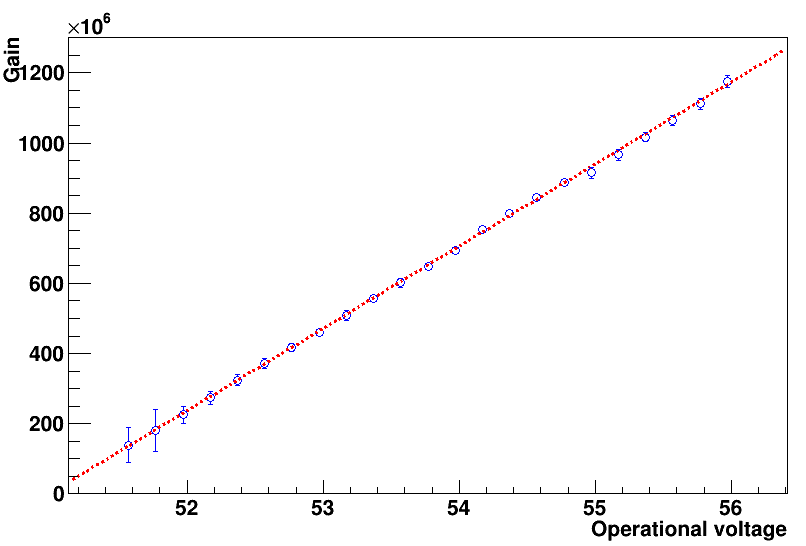
\includegraphics[scale=0.2]{Dependenciavoltaje.png}
\caption{\textbf{Imagen 20}.- Ganancia frente a voltaje operacional}
\end{figure}

Podemos observar de nuevo la existencia de un comportamiento lineal casi perfecto en un rango de voltaje de 5 voltios. Vemos de nuevo reflejada la propiedad de buena linealidad que caracteriza a los SiPM. En la gráfica podemos notar la existencia de un mayor error en las medidas de voltajes mas bajos (en valor absoluto). Esto es debido a que nos estamos acercando al voltaje break down donde el silicio entra en modo Geiger y el valor de la ganancia empieza a ser distinto de cero. Podemos hachacar este mayor error a que a estos voltajes cercanos a la frontera de cambio de comportamiento, el SiPM todavía no funciona de forma adecuada debido a efectos más sutiles. Este necesita estar totalmente dento del modo Geiger para funcionar perfectamente. Hay que tener en cuenta además que solo se llego hasta el voltaje $V_{op}=51,57$ V debido a que, cuando estamos a valores muy cercanos al voltaje de break down la ganancia sufre un decaimiento exponencial, siendo imposible realizar su medida.

\paragraph {}
Podemos observar que, al contrario de lo que ocurría con la temperatura, el valor de la ganancia del SiPM aumenta a medida que aumenta el voltaje operacional. Esto es debido a que....

\paragraph {}
La ecuación obtenida en este ajuste $G=cV_{op}+d$ toma los siguientes valores: 
\begin{itemize}
\item{} $c=2.34123 \cdot 10^8 \pm 2.55246 \cdot 10^6$ $V^{-1}$
\item{} $d=-1.19368 \cdot 10^{10} \pm 1.38112 \cdot 10^8$ $V^{-1}$
\end{itemize}

Remarquemos de nuevo la importancia de este resultado, no por el resultado numérico, sino porque es la parte que nos faltaba para poder calcular la compensación de la ganancia.

\paragraph {}
A demás, a modo de comprobación, podemos obtener el Voltage break down a partir de esta expresión, que se corresponde al voltaje al cual la ganancia es cero (voltage a partir del cual estamos en modo geiger y la ganancia empieza a ser no nula). El voltage calculado es: 
$$G=0=c \cdot V_{BD} +d \longrightarrow V_{BD}=-\frac{d}{c}=50.9852$$

Vemos que este se acerca de forma extraordinaria al voltaje teórico especificado por hamamatsu, 50.97.
\end{itemize}
	
\subsection {Compensación de la ganancia}
\paragraph {}
Finalmente, con toda esta información, procedemos a desarrollar un protocolo de compensación de la ganancia. Nuestro objetivo es que, ante una modificación de la ganancia debido a una variación involuntaria de la temperatura (por ejemplo debido a variación climatológicas) aplicar de manera voluntaria una variación adecuada en el voltaje operacional que devuelva a la ganancia a su valor inicial.

\paragraph {}
Como ya se ha explicado la importancia de este estudio de compensación es poder utilizar este sistema a modo de alarma. Dado que este estará expuesto a condiciones climáticas inevitablemente sufrira variaciones de temperatura. Si queremos el detector final sea capaz de avisar en caso de obtener una señal demasiado grande y que esta señal se corresponda a una fuga de tritio necesitamos que el sistema posea una ganancia constante.

Las expresiones que se han obtenido con las dos calibraciones anteriores son:
$$G(V_{op})=cV_{op}+d; \qquad G(T)=aT+b$$

Esto implica que una variación de la ganancia en cada una de estas magnitudes viene reflejado como:
$$\partial G(V_{op}) = c \partial V_{op}; \qquad \partial G(T) = a \partial T$$

Finalmente, la variación total de la ganancia ante una variación de ambas magnitudes viene dado por:
$$\partial G_{tot} = \partial G(V_{op}) + \partial G(T)$$

Por tanto, si queremos que el valor de la ganancia se conserve ante una variación de ambas magnitudes tendremos que conseguir que: 
$$\partial G_{tot} = 0 =  \partial G(V_{op}) + \partial G(T) \longrightarrow \partial G(V_{op}) = -\partial G(T)  $$

En otras palabras, lo que tenemos que conseguir es producir la misma variación a la ganancia con la modificación del voltaje que la que se ha producido al variar la temperatura. Para determinar esta variarión únicamente sustituimos las expresiones anteriormente obtenidas para cada diferencial de la ganancia:
$$\partial G(V_{op}) = - \partial G(T)  \longrightarrow c \partial V_{op}= - a \partial T \longrightarrow  \partial V_{op}= - \frac{a}{c} \partial T$$

Finalmente consideramos que a y c las consideramos constantes en voltaje y temperatura, ya que, estas varian muy poco por lo que, en primera aproximación, es aceptable. Con ello integramos a cada lado y obtenemos:
$$\int_{V_i}^{V_f} \partial V_{op}= - \frac{a}{c} \int_{T_i}^{T_f}\partial T = - \frac{a}{c} \Delta T \longrightarrow \Delta V_{op}= e \Delta T$$

Donde se ha introducido un nuevo parámetro: $e=-\frac{a}{c}$ cuyo valor es:
$$c=2.34123 \cdot 10^8 \pm 2.55246 \cdot 10^6 \quad V^{-1}$$
$$a=-1.40308 \cdot 10^7 \pm 2.71545 \cdot 10^5 \quad T^{-1}$$
$$e=-\frac{a}{c} = 0.059929 \pm 0,001331$$
Donde el error de e se ha obtenido por propagación de errores. 
\paragraph {}
Finalmente, procedemos a analizar el resultado. Hemos obtenido dos dependencias de la ganancia lineales y opuestas. Por un lado la ganancia disminuye con la temperatura y por otro lado la ganancia aumenta con el voltaje operacional. Por tanto, si queremos conseguir modificaciones opuestas de la ganancia debemos desplazar voltaje y temperatura en la misma dirección (aumentar o disminuir ambas magnitudes simultaneamente). Si analizamos el resultado vemos que, efectivamente tenemos una dependencia positiva.

\paragraph {}
También apreciamos que obtenemos un valor dos ordenes de magnitud inferior a la unidad. Esto es debido a que la dependencia de la ganancia con el voltaje es mucho más marcada que la variación con la temperatura (mayor pendiente en valor absoluto para el ajuste del voltaje que para el ajuste de la temperatura). Este es el motivo por el que se tomo pasos inferiores para el voltaje que para la temperatura. 

\paragraph {}
En resumen la ecuación que nos dicta cual es la variación que debemos aplicar al voltaje para mantener un valor de ganancia constante (compensar la ganancia) ante una variación de la temperatura conocida (que puede ser medida con un sensor de temperatura) es:
$$\Delta V_{op}=0.059929 \cdot \Delta T$$

\paragraph {}
Finalmente tomamos como referencia el caso anteriormente mostrado en la sección de análisis de datos correspondiente a temperatura 25 grados, Humedad del 45\% y voltaje operacional de 53.97 V = $V_{BD}+ 3$ V, cuya ganancia habíamos visto que era $7.18235 \cdot 10^8$ y procedemos a realizar una verificación midiendo los casos de 21, 23, 25, 27 y 29 grados. En cada uno de ellos se corregirá el voltaje de alimentación de forma adecuada para mantener el mismo valor de la ganancia. El valor de la ganancia para cada caso se ve reflejado en la imagen veintiuno. 

\begin{figure}[hbtp]
\centering
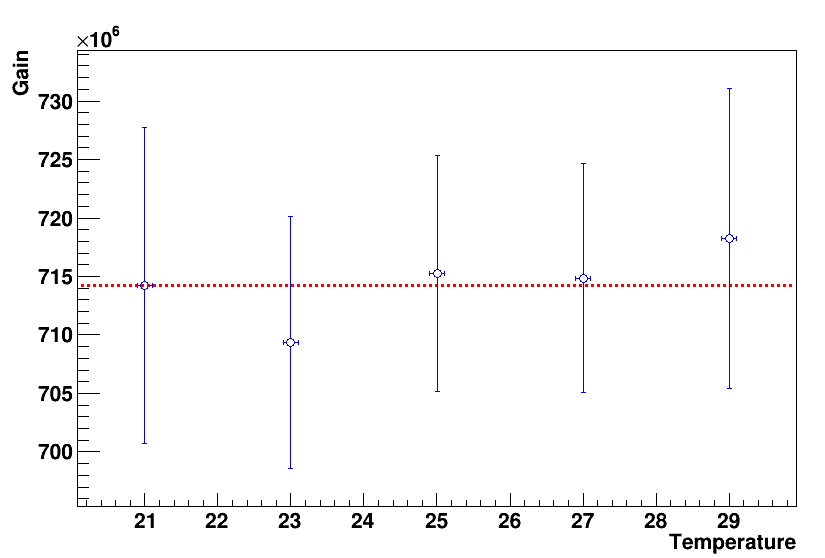
\includegraphics[scale=0.2]{compensacion.png}
\caption{\textbf{Imagen 21}.- Verificación del método de compensación}
\end{figure}

Donde la raya roja corresponde al ajuste a una constante. Su valor, correspondiente al valor de la ganancia es $G=7.14203 \cdot 10^8 \pm 4.97472 \cdot 10^6$

\paragraph {}
Podemos ver que el método funciona de manera muy eficaz ya que la ganancia presenta variaciones muy pequeñas de aproximadamente $\Delta G=5 \cdot 10^6$, que corresponde a una variación relativa del $2.801 \cdot 10^{-3} $. Vemos que es un método realmente eficaz.
\paragraph {}
La máxima variación se observo a 23 grados. Esta es debido a que fue una medida realizada muchas horas despues de tomarse las otras y existen factores externos que no podemos controlar y afectan al sistema. En este tiempo más largo transcurrido es más probable que hayan cambiado estos factores. Sin embargo puede observarse en todo momento que la variación de la ganancia es mínima verificando en gran medida la ecuación anteriormente obtenida.





\section {Protocolo de manipulación de fibras centelleadoras}
\paragraph {}
Para detectar y medir los electrones que se emiten en la desintegración $\beta^-$ del tritio (referencia a la formula de la desintegración del tritio) se utilizarán fibras centelleadoras, en concreto las fibras BCF-12. 

\paragraph {}
Un elemento centelleador esta formado por materiales luminiscentes cuyos átomos o moléculas que los componen presentan unos niveles energéticos similares a los de la imagen veintidos:

\begin{figure}[hbtp]
\centering
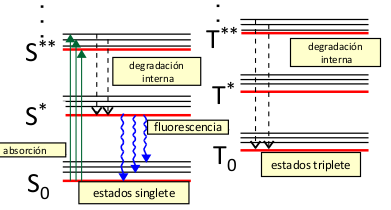
\includegraphics[scale=0.5]{EsquemaNivelesFIbras.png}
\caption{\textbf{Imagen 22}.- Esquema de niveles energéticos}
\end{figure}

Donde los estados S representan singletes y los estados T tripletes. Cuando la radiación ionizante, en nuestro caso los electrones procedentes del tritio, atraviesa el centelleador sus átomos y/o moléculas absorben su energía produciendose una excitación de los mismos. 

\paragraph {}
Posteriormente estos se desexcitan, en primer lugar desde niveles superiores hasta el nivel S* o $T_0$ por degradación interna (en un tiempo del orden del ps) y seguidamente del S* hasta $S_0$ (en un tiempo del orden del ns). En esta segunda desexcitación emitien fotones cuyo rango de longitud de onda puede ir desde el ultravioleta hasta el infrarrojo [100-800]nm dependiendo de la distancia existente entre estos niveles energéticos. 

\paragraph {}
Estos fotones son los que se conocen como fluorescencia y es lo que se utiliza habitualmente como señal de respuesta de un material centelleador. En concreto, en nuestro experimento, esta será la señal que utilizaremos cuyo espectro es el mostrado en la imagen 3.

\paragraph {}
Hay que tener en cuenta que las fibras centelleadoras son transparentes a los fotones que se encuentran en la longitud de onda de su emisión ya que, de lo contrario, tendríamos una nueva reabsorción de los fotones emitidos antes de ser detectados por el contador de fotones, situación indeseada.

\paragraph {}
Los materiales centelleadoras presentan una muy buena linealidad con la energía de la radiación incidente a partir de una energía mínima que determina la sensibilidad del material centelleador utilizado, en nuestro caso... Teniendo en cuenta que el SiPM también presenta una muy buena linealidad con la señal recibida esperamos obtener una señal de nuestro detector que presente una buena linealidad con la energía que pretendamos medir.

\paragraph {}
Por lo general estos materiales centelleadores producen señales bastante rápidas en comparación con otros tipos de detectores tales como.... Utilizamos fibras centelleadoras orgánicas ya que estas son 2 o 3 órdenes de magnitud más rápidas que las inorgánicas,  en concreto las fibras que utilizaremos presentan un tiempo de decaimiento de 3,2 ns. 

\paragraph {}
Además debe de ser capaz de producir el mayor número de fotones por unidad de energía para poder tener un mayor detalle de la señal medida. Las fibras BCF-12 son capaces de producir 8000 fotones por MeV de la radiación incidente. Las fibras BCF-12 presentan una eficiencia de fotodetección teórica de...

\paragraph {}
Para manipular las fibras se vio necesario la utilización de guantes de latex ya que el propio tacto  del personal encargado del tratamiento de las fibras las ensuciaban y, por extensión, la propagación de la luz se veía afectada.

\paragraph {}
Para poder cortar las fibras centelleadoras de forma opticamente aceptable se diseño y construyo una guillotina adecuada la cual puede verse reflejada en la imagen veintitres:

\begin{figure}[htb]
\centering
{
%\subfloat[Espectro de emisión]
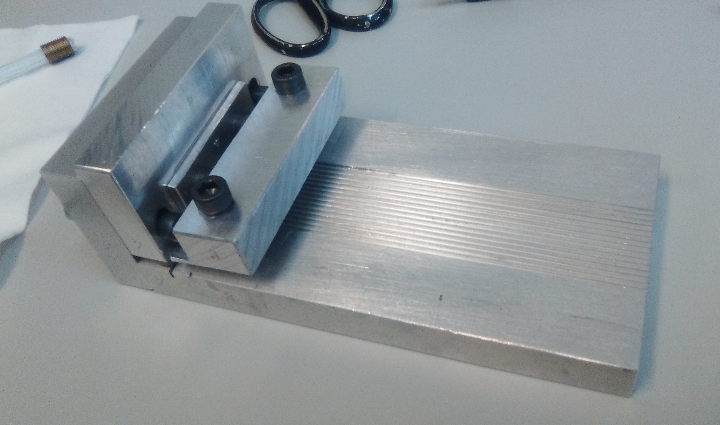
\includegraphics[scale=0.2]{Guillotina1.png} 
}
{
%\subfloat[Espectro de emisión]
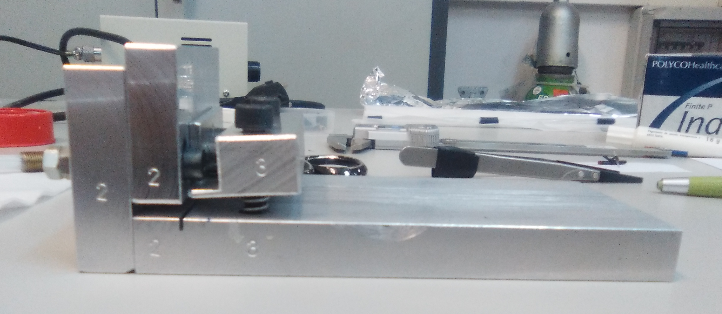
\includegraphics[scale=0.2]{Guillotina2.png} 
}
{
%\subfloat[Espectro de emisión]
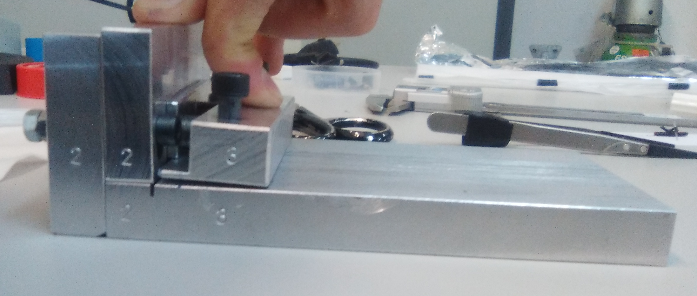
\includegraphics[scale=0.2]{Guillotina3.png} 
}
\caption{\textbf{Imagen 23}.-Guillotina}
\end{figure} 

En la imagen central se puede apreciar que la guillotina disponía de dos piezas independientes (marcadas con los número 2 y 3) las cuales estaban suspendidas por muelles. Para sujetar y cortar cada una de las fibra había que pulsar las piezas 3 y 2 respectivamente según puede apreciarse en la imagen de la derecha. 

\paragraph {} 
También puede apreciarse que la guillotina dispone de 14 rieles cuadrados los cuales servían para sujetar cada una de las fibras y, así, obtener un corte limpio y perpendicular. Aunque la guillotina tenía la posibilidad de realizar cortes simultaneos sobre varias fibras centelleadoras siempre se realizaron cortes sobre una única fibra. De esta forma asegurábamos un mejor acabado.


\paragraph {}
Finalmente se estuvo probando con varios tipos de cuchilla (de distinto grosor y tamaño) y se acabo viendo que una cuchilla típica utilizada en las máquinas de afeitar era suficiente. Esta puede apreciarse en la imagen veinticuatro.

\begin{figure}[htb]
\centering
{
%\subfloat[Espectro de emisión]
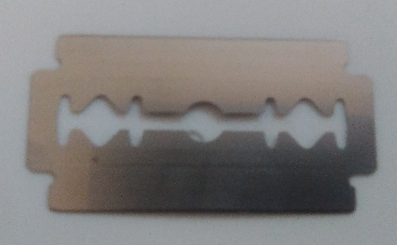
\includegraphics[scale=0.3]{cuchilla.png} 
}
{
%\subfloat[Espectro de emisión]
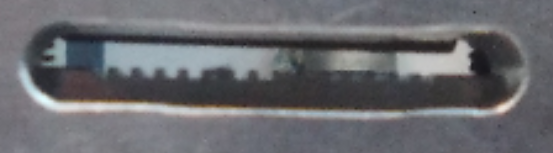
\includegraphics[scale=0.3]{Guillotina5.png} 
}
\caption{\textbf{Imagen 24}.-Cuchilla}
\end{figure} 

\newpage
Hay que tener en cuenta que, para un corte más efectivo se introdujo en la disposición de la cuchilla una lijera inclinación la cual puede apreciarse en la foto de la derecha de la imagen veinticuatro (parte superior del interior del agujero). 

\paragraph {}
En la imagen veinticinco izquierda se puede ver (con ayuda de un microscopio) la cara de una fibra recien cortada. En esta podemos apreciar que, aunque presenta una cabado realmente bueno (sin roturas ni deformaciones) si encontramos que la cara de la fibra se encuentra lijeramente dañada y esto afectaba a la propagación de la luz. La forma de subsanar esto fue pulir cada una de las caras de las fibras. En la parte derecha de la misma imagen podemos observar una foto con la misma fibra trás el proceso de pulido. Podemos comprobar que el simple hecho de pulir las caras de las fibras nos permite obtener fibras con acabado ópticamente aceptable.

\begin{figure}[htb]
\centering
{
%\subfloat[Espectro de emisión]
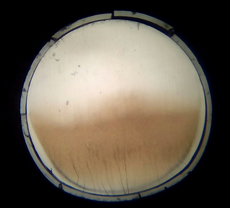
\includegraphics[scale=0.3]{SinPulir.png} 
}
{
%\subfloat[Espectro de emisión]
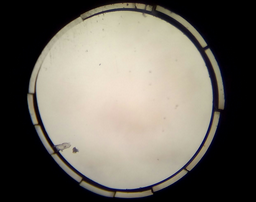
\includegraphics[scale=0.3]{Pulida.png} 
}
\caption{\textbf{Imagen 25}.-Cara fibras}
\end{figure} 

\paragraph {}
Hay que notar en la imagen que el clad aparece roto. Se vío que esto era una característica inevitable del proceso de cortado. Sin embargo pudo observarse que este únicamente se encontraba en el extremo final de la fibra por lo que, la utilización de grasa óptica (marca Saint-Global) para acomplar esta al contador de fotones solucionaba el problema.

\paragraph {}
Seguidamente, con las fibras ya cortadas, simplemente se utilizo un pegamento óptico (marca Saint-Global), especialmente diseñado para materiales centelleadores, para pegarlas entre ellas y obtener, de esta forma, un bunch de fibras. Para que su acabado fuese suficientemente rígido se utilizó un aro metálico en cada uno de los extremos segn la imagúen veintiseis.

\begin{figure}[htb]
\centering
{
%\subfloat[Espectro de emisión]
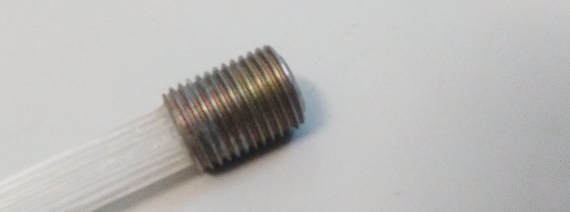
\includegraphics[scale=0.2]{arometalico.png} 
}
{
%\subfloat[Espectro de emisión]

\includegraphics[scale=0.2]{arometalicoconrosca.png} 
}
\caption{\textbf{Imagen 26}.-Aro metálico}
\end{figure} 

En la imagen veintiseis derecha puede apreciarse que este mismo aro disponía de una arandela la cual se utilizaba para una completa sujeción al prototipo.



\paragraph {}
Finalmente, cuando se había secado el pegamento, volvíamos a pulir cada una de las caras del bunch de fibras con el objetivo de obtener una cara total plana (todas las fibras al mismo nivel) para obtener el mejor acomplamiento con el contador de fotones (ya sea SiPM o PMT). En la imagen veintisiete podemos observar un buch de fibras totalmente acabado.

\begin{figure}[htb]
\centering
{
%\subfloat[Espectro de emisión]
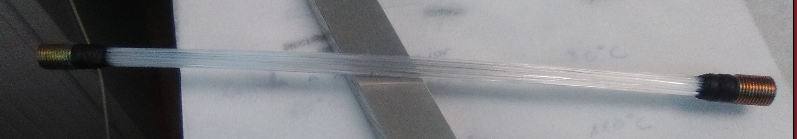
\includegraphics[scale=0.2]{bunchfibras.png} 
}
{
%\subfloat[Espectro de emisión]
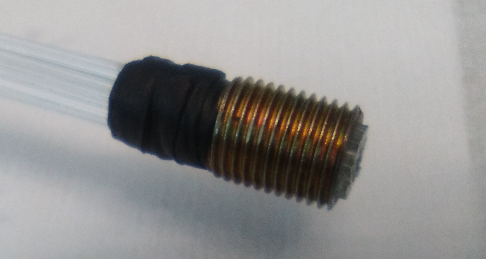
\includegraphics[scale=0.2]{bunchfibras1.png} 
}
\caption{\textbf{Imagen 27}.-Bunch fibras}
\end{figure} 

Este bunch construido disponía de 35 fibras ya que era el mayor número de fibras que cabían en el interior del aro metálico y tenía una extensión máxima de aproximadamente 25 cm, extensión acorde con el prototipo. En la imagen veintiseis derecha podemos apreciar la cara final pulida perfectamente plana. Hay que tener en cuenta que cualquier irregularidad inferior al milímetro en la cara final de bunch era subsanada por el hecho de utilizar grasa óptica para acoplar el bunch de fibra al contador de fotones.



\section {Prototipos} 
	\subsection {Configuración} 
	%Como el tritio tiene un periodo de semidesintegración de 12.32 años podemos hacer un prototipo, y dejarlo ahí para realizar 	todo el estudio. Su actividad no disminuira de manera apreciable
	\subsection {resultados}
\paragraph {}
C

\section {Simulaciones}
\paragraph {}
C

\section {Conclusiones}
\paragraph {}
NOTAS:
\begin{itemize}
\item{} Posible estudio de utilización de método alternativo al WLS para la modificación de la energía de los fotones. Estudiar posibilidad de conseguir scattering elastico a esas energías.
\item {} Punto inacabado= posible estudio de los niveles energéticos del $3^He$ para poder determinar con exactitud la energía de los fotones procedentes de la desexcitación del $3^He$ generado tras la desintegración del tritio.
\item {} Para una compensación en más detalle podríamos estudiar la dependencia de a y c con temperatura y voltaje
\end{itemize}

\section {Agradecimientos}













\newpage
%\section {Bibliografía}
\begin{thebibliography}{99}
\bibitem{Ivo} \textsc{Ivo van Vulpen} y \textsc{Ivan Angelozzi},
\textit{The Standard Model Higgs Boson}
\bibitem{JI} \textsc{José Ignacio Illana},
\textit{EL MODELO ESTÁNDAR Y SU FENOMENOLOGÍA}
\bibitem{notas} \textsc{Siannah Peñaranda Rivas},
\textit{"Quantum Field Theory" Photons and the electromagnetic field}
\bibitem{resumen} \textsc{M. Gomez-Bock}, \textsc{M. Mondragón}, \textsc{M. Mühlleitner}, \textsc{R. Noriega-Papaqui}, \textsc{I. Pedraza}, \textsc{M. Spira} y \textsc{P.M. Zerwas},
\textit{Rompimiento de la simetría electrodébil y la física del Higgs: Conceptos Básicos}
\bibitem{Martin} \textsc{Francis Halzen} y \textsc{Alan D. Martin},
\textit{QUARKS AND LEPTONS: An Introductory Course in Modern Particle Physics}
\bibitem{PDG} \textit{Partícle data group} (http://pdg.lbl.gov/)
\bibitem{QCD} \textsc{Matthias Jamin},
\textit{QCD and Renormalisation Group Methods}
\bibitem{Rojo}\textsc{Juan Rojo},
\textit{The Strong Interaction and LHC phenomenology}
\bibitem{Thomson} \textsc{Mark Thomson},
\textit{Particle Physics}
\bibitem{notas1} \textsc{Mark Thomson},
\textit{Particle Physics} Handout 1: Introducción
\bibitem{notas2} \textsc{Mark Thomson},
\textit{Particle Physics} Handout 1: Symmetries and Quark Model
\bibitem{Santos} \textsc{Joaquín Santos Blasco},
\textit{UNITARY ANALYSIS OF THE SCALAR SECTOR OF THE STANDARD MODEL}
\bibitem{string} \textsc{J. Marsano},
\textit{String Thery in the LHC Era} Lecture 3: Why do we need the Higgs? 

\end{thebibliography}

\end {document}